\section{z-transform}

We will study the asymptotic behavior of the approximate risk\[r_t = \frac{1}{2} \sum_{i=1}^d Li^{-\alpha} \left( m_{0,i} \prod_{j=0}^{t-1} \left[ (1-\eta_j Li^{-\alpha})^2+2\eta_j^2 L^2 i^{-2\alpha} \right] + \sum_{k=0}^{t-1} \eta_k^2 \sigma^2 Li^{-\alpha} \prod_{j=k+1}^{t-1} \left[ (1-\eta_j Li^{-\alpha})^2+2\eta_j^2 L^2 i^{-2\alpha} \right] \right)\]using z-transforms and Laplace's method.



\subsection{$\eta_t$ constant}

Let us compute the z-transform $R(z)$ of the approximate risk $(r_t)_t$ (cf. \ref{eq:approx}).
\[
R(z) = R_1(z) + R_2(z)
\]

Let $\tilde A =  (1-\eta\Lambda)^2+2\eta^2 \Lambda^2$

$\tilde A = \diag(a)$ with $a_i = (1-\eta\lambda_i)^2+2\eta^2 \lambda_i^2$

\begin{align*}
\bullet R_2(z)= \sum_{t=0}^{\infty} \frac{1}{2} \sum_{k=0}^{t-1} \eta^2 \sigma^2 \langle \lambda, \tilde A^k \lambda \rangle z^t 
&= \sum_{k=0}^{\infty} \sum_{t=k+1}^{\infty} \frac{\eta^2 \sigma^2}{2} \langle \lambda, \tilde A^k \lambda \rangle z^t \\
&= \sum_{k=0}^{\infty} \frac{\eta^2 \sigma^2}{2} \langle \lambda, \tilde A^k \lambda \rangle \frac{z^{k+1}}{1-z} \\
&= \frac{z}{1-z} \sum_{k=0}^{\infty} \frac{\eta^2 \sigma^2}{2} \langle \lambda, \tilde A^k \lambda \rangle z^k\\
&=\frac{z}{1-z} \sum_{i=0}^{\infty} \frac{\eta^2 \sigma^2}{2} \lambda_i^2 \frac{1}{1-a_iz}
\end{align*}


\[
\bullet R_1(z)=\sum_{t=0}^{\infty} \frac{1}{2} \langle \lambda, \tilde A^t m_0 \rangle z^t = \sum_{i=0}^{\infty} \frac{1}{2} \lambda_i m_{0i} \frac{1}{1-a_iz}
\]

\[ R(z)=\frac{1}{2} \sum_{i=0}^{\infty}  \frac{\lambda_i m_{0i}}{1-a_iz} +  \frac{\eta^2 \sigma^2 \lambda_i^2 z}{(1-z)(1-a_iz)}
\]

Therefore $\displaystyle \lim_{t\to \infty} r_t =  \lim_{z\to 1^-} (1-z) R(z) = \frac{1}{2}\sum_{i=0}^\infty    \frac{\eta^2 \sigma^2 \lambda_i^2}{1-a_i}$



\subsection{Linear decay [WRONG]}

Let $s_T$ be the risk after $T$ iterations for a linear decay $\eta_{j}^{(T)} = \eta\frac{T-j}{T}$

Let $a_{t,i}^{(T)} = \left[ 1 - 2 \frac{T-t}{T} \frac{L\eta}{i^\alpha} + 3 \left( \frac{T-t}{T} \frac{L\eta}{i^\alpha} \right)^2 \right]$


The z-transform of $(s_t)$ is $\sum_i S_i$ where
\[
S_i(z) = \frac{1}{2} \frac{L}{i^\alpha}\sum_{T=0}^{\infty} \left( \prod_{t=0}^{T-1} a_{t,i}^{(T)} \frac{\Delta}{i^\beta} + \sum_{k=0}^{T-1} \left( \eta \frac{T-k}{T} \right)^2 \frac{L\sigma^2}{t^\alpha} \prod_{j=k+1}^{T-1} a_{j,i}^{(T)} \right) z^T
\]


% Here we consider $\eta_t =(1- \frac{t}{T+1}) \eta$

% \[
% r_{t+1, i} = a_t^i r_{t, i} + \eta_t^2 \sigma^2 \lambda_i^2
% \]

% where $a_t^i = (1 - \eta_t \lambda_i)^2 + 2\eta_t^2 \lambda_i^2$. 
% By substituting the linear schedule into $a_t^i$,

% $$a_t^i = A_i + B_i t + C_i t^2$$

% where the constant coefficients $A_i$, $B_i$, and $C_i$ are defined as:
% \begin{align*}
% A_i &= (1 - \eta \lambda_i)^2 + 2\eta^2 \lambda_i^2 \\
% B_i &= \frac{2\eta\lambda_i(1 - \eta\lambda_i) - 4\eta^2\lambda_i^2}{T+1} = \frac{2\eta\lambda_i - 6\eta^2\lambda_i^2}{T+1} \\
% C_i &= \frac{3\eta^2\lambda_i^2}{(T+1)^2}
% \end{align*}
% Then
% \[
% r_{t+1, i} = A_i r_{t, i} + B_i (t  r_{t, i}) + C_i (t^2  r_{t, i}) + \eta^2\sigma^2\lambda_i^2 (1-\tfrac{t}{T+1})^2
% \]


% Therefore

% \[
% \frac{1}{z}(R_i(z)-r_{0i}) = A_iR_i(z) + B_i z R_i'(z) +C_i(zR_i'(z) + z^2 R_i''(z)) + D_i
% \]
% with $D_i = \sum_{t=0}^T \eta^2\sigma^2\lambda_i^2 (1-\frac{t}{T+1})^2z^t$


% PROBLEM?: here the z transform is useful only if $T= \infty$, which is impossible for a linear decay.

% \begin{figure}[h]
% \centering
% 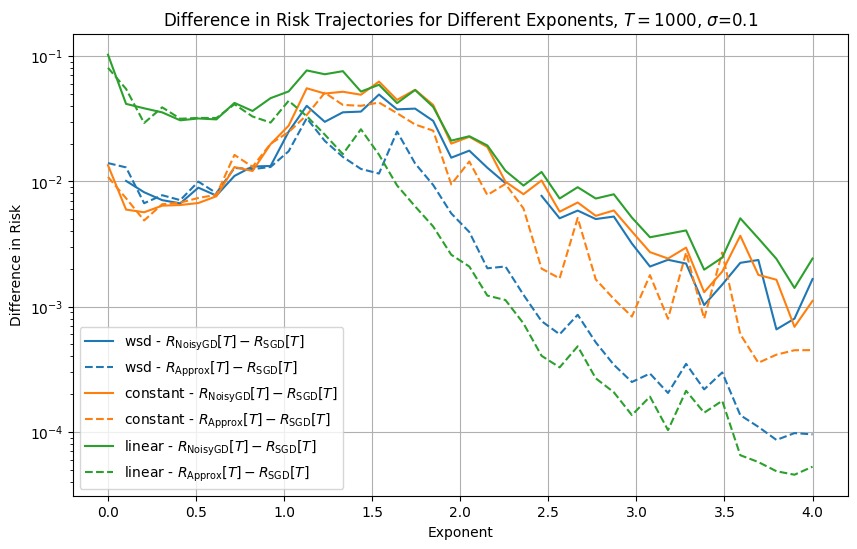
\includegraphics[width=0.7\textwidth]{images/exponents_to_risks.png}
% \caption{$\sigma = 0.1$}
% \label{fig:figure2}
% \end{figure}


% \begin{figure}[h]
% \centering
% 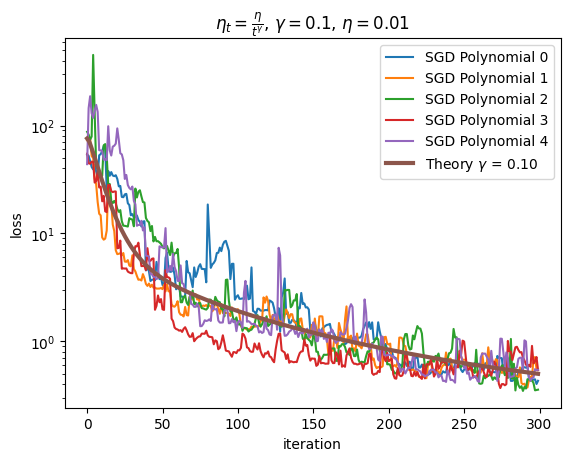
\includegraphics[width=0.7\textwidth]{images/polynomial_test.png}
% \caption{Theory and simulations with $\eta_t = \frac{\eta}{t^\gamma}$}
% \label{fig:figure2}
% \end{figure}



